\documentclass[11pt]{article}

\usepackage[margin=1in]{geometry}
\usepackage[utf8]{inputenc}
\usepackage[T1]{fontenc}
\usepackage{lmodern}
\usepackage{microtype}
\usepackage{graphicx}
\usepackage{booktabs}
\usepackage{amsmath, amssymb}
\usepackage{array}
\usepackage{longtable}
\usepackage{float}
\usepackage[hidelinks]{hyperref}
\usepackage{xcolor}
\usepackage{listings}
\usepackage{caption}
\usepackage{lineno}
\linenumbers

\captionsetup{font=small,labelfont=bf}

\lstset{
  basicstyle=\ttfamily\small,
  breaklines=true,
  frame=single,
  backgroundcolor=\color{gray!10}
}

\title{\textbf{Supplementary Information}\\
\large OmniGene-4: A Unified Bio-Language MoE Model with Router-Level Interpretability}

\author{Liang Wang\\
\small School of Artificial Intelligence and Automation\\
\small Huazhong University of Science and Technology}

\date{}

\begin{document}

\maketitle
\tableofcontents
\newpage

%% ============================================================
\section{Supplementary Note 1: Extended Limitations and Future Work}
%% ============================================================

\paragraph{Top-1 expert purity is modest.} The highest-purity atomic expert we identified (E54, English function-words at layer 12) reaches 80\%, but most ``specialty'' experts land at 15--35\% purity. Our claims about task-specific experts should be understood distributionally rather than as hard assignments.

\paragraph{Single model family.} All results are from Gemma-4-26B-A4B-Instruct. Whether the 96\%/4\% CPT/SFT decomposition generalizes to Mixtral, DeepSeek-MoE, or GPT-class bio models is an open question. The architectures differ in expert count, top-$k$ selection, and router objective.

\paragraph{Remote-homology ceiling.} Our 82.60\% remote-homology accuracy leaves an 18\% error rate. Specialist methods with structural-alignment heads (ESM-2 + TM-Vec, PLMSearch, CATHe) report 65--75\% on differently constructed splits. We hypothesize the remaining gap is a representation-level constraint rather than an SFT-scale constraint; testing requires controlled experiments with more CPT on distant-protein pairs ($\approx$150 GPU-hours, deferred).

\paragraph{No chain-of-thought reasoning.} We briefly attempted to train with \texttt{<THOUGHT>} reasoning blocks for remote homology but abandoned it because synthetic-CoT templates from sequence features were of insufficient quality. Human-expert or strong-teacher-generated CoT data would likely improve remote-homology performance substantially.

\paragraph{Evaluation scale.} BixBench's True/False subset contains only $\approx$200 questions; small absolute differences in the 90--95\% range are within the dataset's noise floor. Richer evaluation pools (HELM-Bio, LM-BIO) would strengthen the claims.

\paragraph{No ablation on \texttt{router.proj} LoRA.} We state that including \texttt{router.proj} in the LoRA target modules is critical to enabling expert re-specialization, based on an informal pilot observation. A controlled ablation --- CPT with and without \texttt{router.proj} LoRA, holding all other hyperparameters fixed --- would quantify this claim.

\paragraph{Future experiments.} (1) Controlled CPT ablation with richer distant-protein corpora. (2) Router.proj ablation. (3) Human-expert CoT for remote homology. (4) Replication on Mixtral-8x7B or DeepSeek-MoE-16B. (5) Downstream wet-lab validation (variant effect prediction on ClinVar). (6) GGUF quantization for single-GPU deployment on RTX 4090.

%% ============================================================
\section{Supplementary Tables}
%% ============================================================

\subsection{Supplementary Table S1: Full Per-Layer JS Divergence}

\begin{longtable}{lcccc}
\caption{Layer-by-layer Jensen--Shannon divergence across training stages. Values are mean pairwise JS across all 28 task pairs at each layer.}\\
\toprule
\textbf{Layer} & \textbf{Baseline} & \textbf{CPT} & \textbf{v3 (CPT+SFT)} & \textbf{$\Delta$ CPT} \\
\midrule
\endfirsthead
\multicolumn{5}{c}{\tablename\ \thetable\ -- \textit{Continued}} \\
\toprule
\textbf{Layer} & \textbf{Baseline} & \textbf{CPT} & \textbf{v3 (CPT+SFT)} & \textbf{$\Delta$ CPT} \\
\midrule
\endhead
\bottomrule
\endlastfoot
0  & 0.160 & 0.164 & 0.164 & +0.004 \\
1  & 0.136 & 0.113 & 0.113 & $-$0.023 \\
2  & 0.172 & 0.164 & 0.164 & $-$0.008 \\
3  & 0.151 & 0.134 & 0.134 & $-$0.017 \\
4  & 0.119 & 0.113 & 0.113 & $-$0.006 \\
5  & 0.159 & 0.160 & 0.160 & +0.001 \\
6  & 0.131 & 0.111 & 0.111 & $-$0.020 \\
7  & 0.129 & 0.123 & 0.123 & $-$0.006 \\
8  & 0.134 & 0.126 & 0.126 & $-$0.008 \\
9  & 0.174 & 0.153 & 0.153 & $-$0.021 \\
10 & 0.197 & 0.159 & 0.159 & $-$0.038 \\
11 & 0.160 & 0.143 & 0.143 & $-$0.017 \\
12 & 0.182 & 0.149 & 0.149 & $-$0.033 \\
13 & 0.143 & 0.127 & 0.127 & $-$0.016 \\
14 & 0.157 & 0.137 & 0.137 & $-$0.020 \\
15 & 0.198 & 0.170 & 0.170 & $-$0.028 \\
16 & 0.139 & 0.121 & 0.121 & $-$0.018 \\
17 & 0.184 & 0.166 & 0.166 & $-$0.018 \\
18 & 0.148 & 0.134 & 0.134 & $-$0.014 \\
19 & 0.124 & 0.123 & 0.123 & $-$0.001 \\
20 & 0.140 & 0.130 & 0.130 & $-$0.010 \\
21 & 0.136 & 0.119 & 0.119 & $-$0.017 \\
22 & 0.162 & 0.149 & 0.149 & $-$0.013 \\
23 & 0.157 & 0.138 & 0.138 & $-$0.019 \\
24 & 0.141 & 0.122 & 0.122 & $-$0.019 \\
25 & 0.180 & 0.149 & 0.149 & $-$0.031 \\
26 & 0.161 & 0.152 & 0.152 & $-$0.009 \\
27 & 0.178 & 0.172 & 0.172 & $-$0.006 \\
28 & 0.217 & 0.197 & 0.197 & $-$0.020 \\
29 & 0.240 & 0.222 & 0.222 & $-$0.018 \\
\end{longtable}

\subsection{Supplementary Table S2: Bootstrap Confidence Intervals}

\begin{table}[H]
\centering
\caption{Bootstrap 95\% confidence intervals for routing metrics (1,000 prompt-level iterations).}
\begin{tabular}{lccc}
\toprule
\textbf{Metric} & \textbf{Mean} & \textbf{95\% CI Lower} & \textbf{95\% CI Upper} \\
\midrule
Baseline JS & 0.344 & 0.344 & 0.344 \\
CPT JS & 0.440 & 0.440 & 0.441 \\
v3 JS & 0.444 & 0.444 & 0.444 \\
$\Delta$ CPT & 0.096 & 0.096 & 0.097 \\
$\Delta$ SFT & 0.004 & 0.003 & 0.004 \\
\bottomrule
\end{tabular}
\end{table}

\subsection{Supplementary Table S3: Format-Matched Routing Control}

\begin{table}[H]
\centering
\caption{Layer-averaged JS divergence before and after format matching. Six tasks wrapped in a neutral template (\texttt{\#\#\# Task: \{name\} / \#\#\# Content: \{text\} / \#\#\# End}).}
\begin{tabular}{lcc}
\toprule
\textbf{Condition} & \textbf{JS Divergence} & \textbf{Retention Ratio} \\
\midrule
Original (heterogeneous formats) & 0.160 & 100\% \\
Format-matched (neutral template) & 0.145 & 90.2\% \\
\bottomrule
\end{tabular}
\end{table}

\subsection{Supplementary Table S4: Head-to-Head Baseline Comparison (Full)}

\begin{table}[H]
\centering
\small
\caption{Remote homology accuracy on identical 500-pair balanced evaluation (\texttt{protein\_pair\_remote}, seed 42). All methods evaluated on the same pair set.}
\begin{tabular}{lcccc}
\toprule
\textbf{Method} & \textbf{Type} & \textbf{Acc (default)} & \textbf{Acc (optimal)} & \textbf{ROC AUC} \\
\midrule
ESM-2 650M & PLM (mean-cosine) & 50.50\% & 51.80\% & 0.513 \\
ESM-2 3B   & PLM (mean-cosine) & 50.00\% & 51.20\% & 0.512 \\
MMseqs2 (easy-search, $s$=7.5) & alignment & 54.40\% & 55.60\% & 0.556 \\
DIAMOND (more-sensitive)     & alignment & 53.20\% & 53.20\% & 0.532 \\
Gemma-4-Instruct (vocab-ext, ZS) & LM (chat) & 60.00\% & --- & --- \\
\midrule
OmniGene-4 v3 & LM (chat) & 59.50\% & --- & --- \\
OmniGene-4 v4 & LM (chat) & 82.00\% & --- & --- \\
\textbf{OmniGene-4 v5} & LM (dual-head) & \textbf{82.60\%} & --- & --- \\
\bottomrule
\end{tabular}
\end{table}

\subsection{Supplementary Table S5: Multi-task Generation Evaluation (v5)}

\begin{table}[H]
\centering
\caption{Multi-task generation accuracy across six evaluation categories, 100 samples each, on a held-out split. Keyword-overlap is the standard text-overlap score; Structure additionally reports character-level overlap on the 3Di/DSSP output strings.}
\begin{tabular}{lcc}
\toprule
\textbf{Category} & \textbf{Keyword score} & \textbf{Char overlap} \\
\midrule
Protein     & 1.000 & --- \\
Mol         & 0.980 & --- \\
Cell        & 0.966 & --- \\
Literature  & 0.559 & --- \\
Mutation    & 0.113 & --- \\
Structure (gen mode) & 0.000 & 0.259 \\
\bottomrule
\end{tabular}
\end{table}

\subsection{Supplementary Table S6: Per-residue Classification Head Accuracy (v5)}

\begin{table}[H]
\centering
\caption{Per-residue accuracy of the two classification heads on a 50-protein held-out evaluation, under teacher-forced reference-residue inference.}
\begin{tabular}{lcccc}
\toprule
\textbf{Head} & \textbf{Classes} & \textbf{Chance} & \textbf{Accuracy} & \textbf{N proteins} \\
\midrule
3Di (Foldseek)        & 20 & 5.0\%  & 78.6\%  & 19 \\
DSSP (secondary str.) & 8  & 12.5\% & 100.0\% & 31 \\
\bottomrule
\end{tabular}
\end{table}

\subsection{Supplementary Table S7: SFT Hyperparameters Across All Stages}

\begin{table}[H]
\centering
\small
\caption{SFT hyperparameters. v2/v3 used a chat-style template; v4 switched to pure Alpaca with loss masking and task oversampling. v5 adds dual-head classifiers trained jointly with generation.}
\begin{tabular}{lccc}
\toprule
\textbf{Parameter} & \textbf{v2 / v3} & \textbf{v4} & \textbf{v5} \\
\midrule
Init from & v2 / Gemma-bio & v3 LoRA + embed & v4 LoRA + embed \\
Training data & 179K / 199K instr & 199K (resampled) & $\sim$21K Structure \\
Prompt template & chat tags & pure Alpaca & pure Alpaca \\
Loss masking & no & yes ($-100$) & yes ($-100$) \\
Joint loss & gen CE only & gen CE only & 0.5 gen + 0.5 cls \\
Effective batch & 64 & 64 & 32 \\
Learning rate & 5e-5 / 2e-5 & 2e-5 & 1e-5 \\
Sequence length & 1024 & 1536 & 1536 \\
Steps & 3,118 / 3,118 & 4,257 & 1,350 \\
GPU-hours & 11.8 / 13.2 & $\sim$30 & $\sim$5 \\
\bottomrule
\end{tabular}
\end{table}

\subsection{Supplementary Table S8: Case-Study Pair Details}

\begin{table}[H]
\centering
\small
\caption{Five case-study protein pairs. ESM2 columns: binary prediction at cosine threshold 0.5. MMseqs/DIAMOND: 1 if hit found at E$\leq 10^{-3}$, 0 otherwise. v5: parsed answer. Y = correct, N = wrong.}
\begin{tabular}{c c r r c c c c c c}
\toprule
\textbf{Case} & \textbf{Type} & \textbf{Len1} & \textbf{Len2} & \textbf{Label} & \textbf{ESM-650} & \textbf{ESM-3B} & \textbf{MMseqs} & \textbf{DIAM} & \textbf{v5} \\
\midrule
1 & A & 107 & 106 & 1 & 1(Y) & 1(Y) & 0(N) & 0(N) & 1(Y) \\
2 & A & 142 & 161 & 1 & 1(Y) & 1(Y) & 0(N) & 0(N) & 1(Y) \\
3 & B & 244 & 157 & 0 & 1(N) & 1(N) & 0(Y) & 0(Y) & 0(Y) \\
4 & C & 143 & 101 & 1 & 1(Y) & 1(Y) & 1(Y) & 1(Y) & 1(Y) \\
5 & D & 108 & 176 & 1 & 1(Y) & 1(Y) & 0(N) & 0(N) & 0(N) \\
\bottomrule
\end{tabular}
\end{table}

\subsection{Supplementary Table S9: Layer-12 Top-3 Routed Experts per Case}

\begin{table}[H]
\centering
\caption{Top-3 routed experts at layer 12 for each case-study pair. The same expert set $\{E_{50}, E_9, E_{108}\}$ activates on all five cases, supporting the conclusion that homology decisions occur inside expert computation rather than at the routing gate.}
\begin{tabular}{c c c c c}
\toprule
\textbf{Case} & \textbf{Outcome} & \textbf{Top-1} & \textbf{Top-2} & \textbf{Top-3} \\
\midrule
1 & v5 correct   & E50 & E9  & E39  \\
2 & v5 correct   & E50 & E9  & E108 \\
3 & v5 correct   & E50 & E9  & E108 \\
4 & v5 correct   & E50 & E108 & E9  \\
5 & v5 wrong     & E50 & E108 & E9  \\
\bottomrule
\end{tabular}
\end{table}

\noindent Layer-12 entropy is stable across cases ($H = 2.70$--$2.83$), and per-layer JS divergence between any homologous case and the non-homologous Case 3 stays below 0.04 across all 30 layers (peak at layer 5, 0.040). For comparison, the layer-averaged cross-task JS is 0.230 (Table S1). The $>$5$\times$ difference supports the gate-vs-expert interpretation in the main text.

\subsection{Supplementary Table S10: Per-Task Entropy Analysis}

\begin{table}[H]
\centering
\caption{Shannon entropy of expert distributions at layer 12 across training stages. Lower entropy = more concentrated expert use.}
\begin{tabular}{lccc}
\toprule
\textbf{Task} & \textbf{Baseline} & \textbf{CPT} & \textbf{v3 (CPT+SFT)} \\
\midrule
NL & 3.85 & 4.13 & 4.15 \\
DNA & 2.89 & 2.76 & 2.78 \\
Protein & 2.76 & 2.54 & 2.56 \\
StdHomology & 2.68 & 2.48 & 2.50 \\
RemHomology & 2.71 & 2.52 & 2.54 \\
Cell & 2.95 & 2.88 & 2.90 \\
Mol & 3.02 & 2.95 & 2.97 \\
Structure & 2.82 & 2.65 & 2.67 \\
\bottomrule
\end{tabular}
\end{table}

\subsection{Supplementary Table S11: Token-Level Expert Specialization at Layer 12}

\begin{table}[H]
\centering
\caption{Top-5 tokens for selected experts at layer 12 (v3 model). Purity = fraction of that expert's activations coming from the dominant modality.}
\begin{tabular}{clp{8cm}}
\toprule
\textbf{Expert} & \textbf{Purity} & \textbf{Top-5 Tokens} \\
\midrule
E54 & 80\% & \texttt{the}, \texttt{of}, \texttt{and}, \texttt{to}, \texttt{in} \\
E59 & 46\% & \texttt{AA}, \texttt{AT}, \texttt{TT}, \texttt{GG}, \texttt{CC} \\
E78 & 35\% & \texttt{M}, \texttt{L}, \texttt{V}, \texttt{I}, \texttt{F} \\
E97 & 28\% & \texttt{CD4}, \texttt{CD8}, \texttt{IL}, \texttt{TNF}, \texttt{IFN} \\
E100 & 15\% & \texttt{(}, \texttt{)}, \texttt{=}, \texttt{C}, \texttt{O} \\
\bottomrule
\end{tabular}
\end{table}

%% ============================================================
\section{Supplementary Figures}
%% ============================================================

\subsection{Supplementary Figure S1: Per-Layer JS Curves}

\begin{figure}[H]
\centering
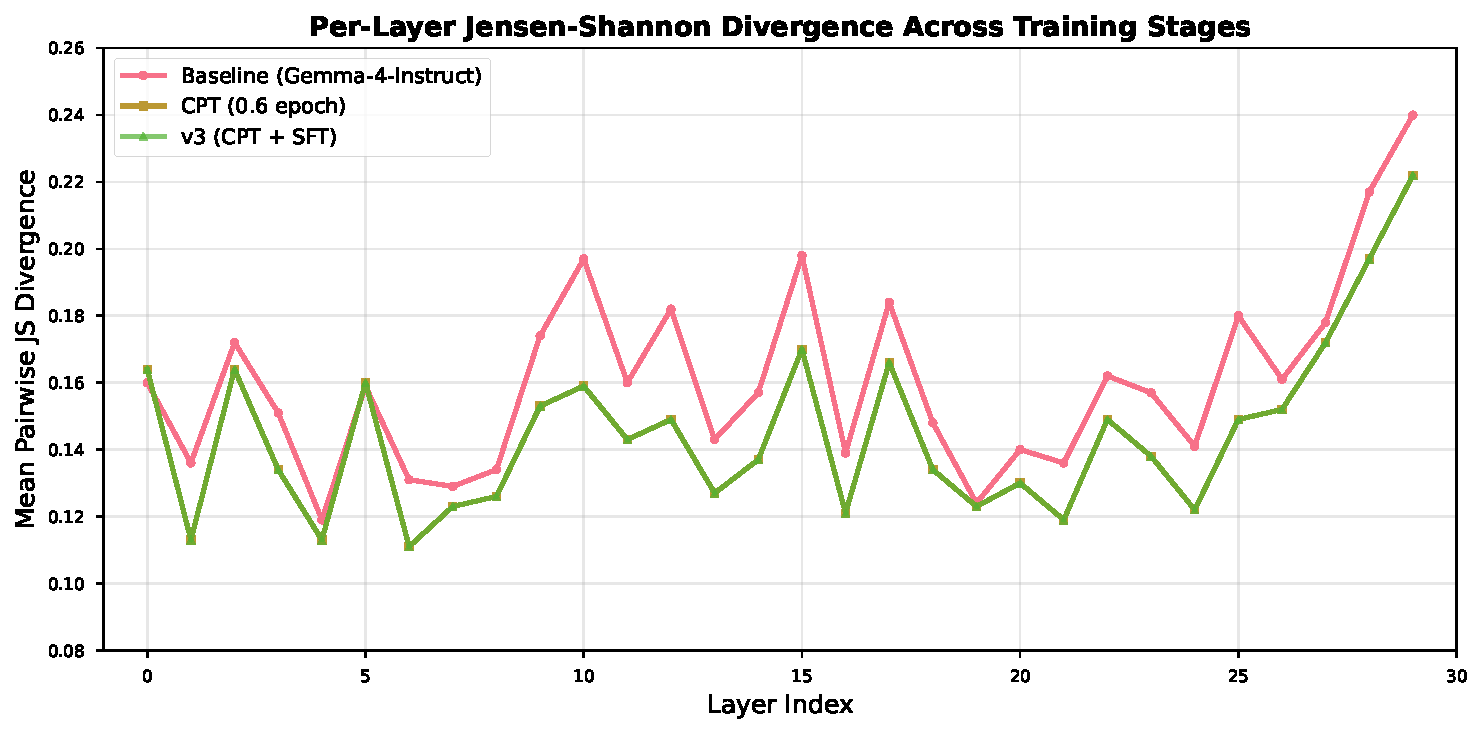
\includegraphics[width=0.95\textwidth]{figures/supp_fig_s1_per_layer_js.pdf}
\caption{Layer-by-layer Jensen--Shannon divergence across training stages. CPT shows the largest increase in middle layers ($L_{11}$--$L_{22}$), while SFT shows concentrated changes near the output layers ($L_{28}$--$L_{29}$).}
\end{figure}

\subsection{Supplementary Figure S2: Expert Activation Heatmap}

\begin{figure}[H]
\centering
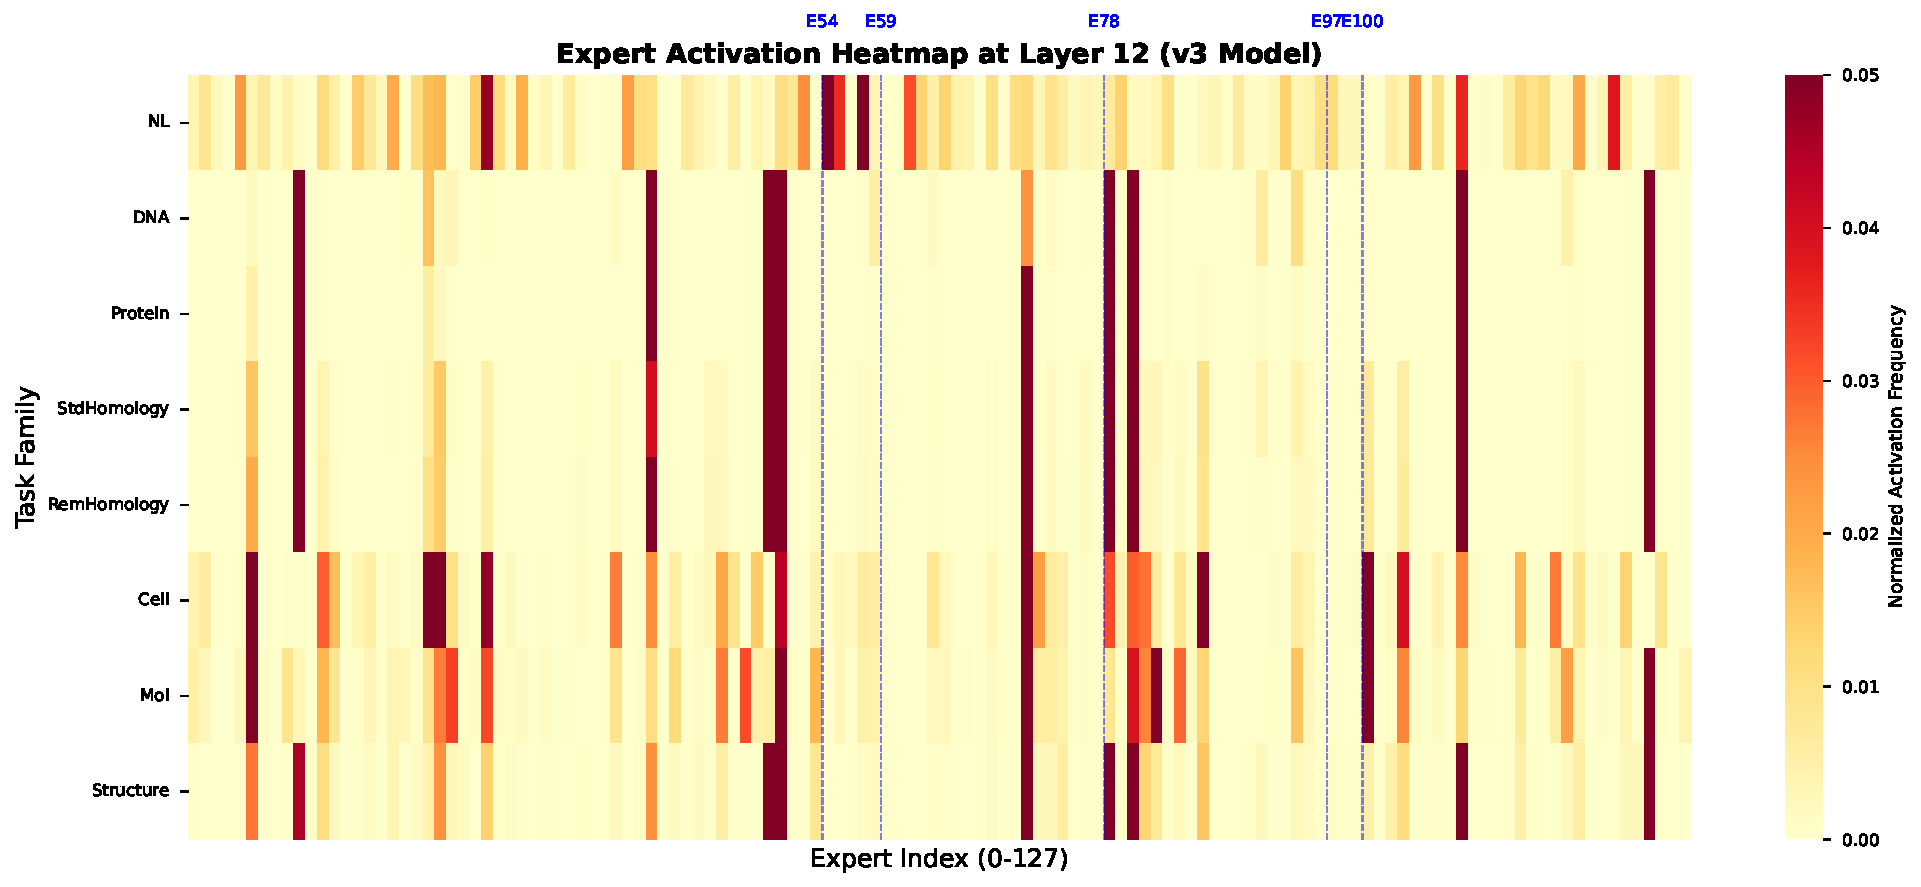
\includegraphics[width=0.95\textwidth]{figures/supp_fig_s2_expert_heatmap.pdf}
\caption{Expert activation heatmap at layer 12 for eight task families. Rows: tasks. Columns: 128 experts. Color intensity indicates normalized activation frequency. Blue dashed lines mark key experts (E54: English function words, E59: DNA 2-mers, E78: amino acids, E97: cell markers, E100: SMILES punctuation).}
\end{figure}

\subsection{Supplementary Figure S3: Bootstrap Distribution}

\begin{figure}[H]
\centering
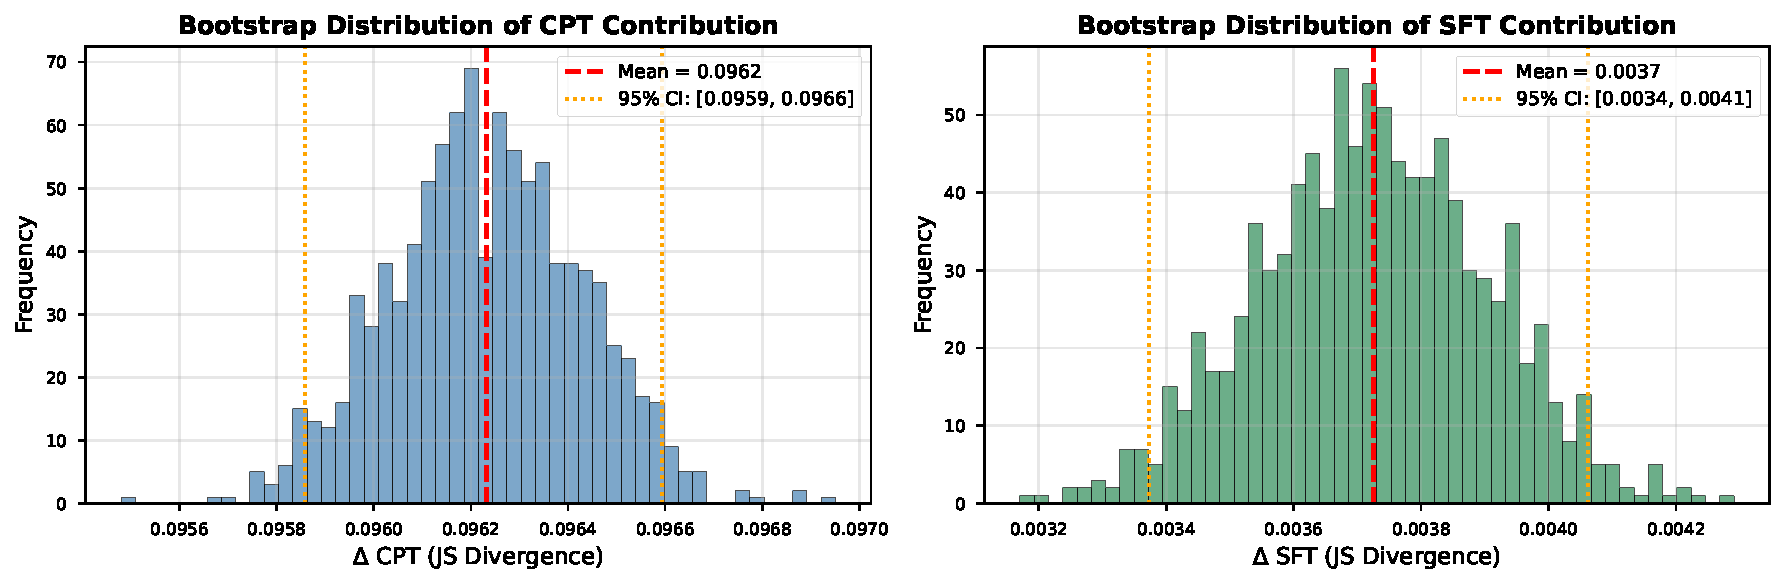
\includegraphics[width=0.95\textwidth]{figures/supp_fig_s3_bootstrap_dist.pdf}
\caption{Bootstrap distribution of CPT and SFT contributions to JS divergence (1,000 iterations). Both distributions are narrow and exclude zero. Left: $\Delta$ CPT = 0.096 [0.096, 0.097]. Right: $\Delta$ SFT = 0.004 [0.003, 0.004].}
\end{figure}

\subsection{Supplementary Figure S4: Case-Study Routing Mosaic}

\begin{figure}[H]
\centering
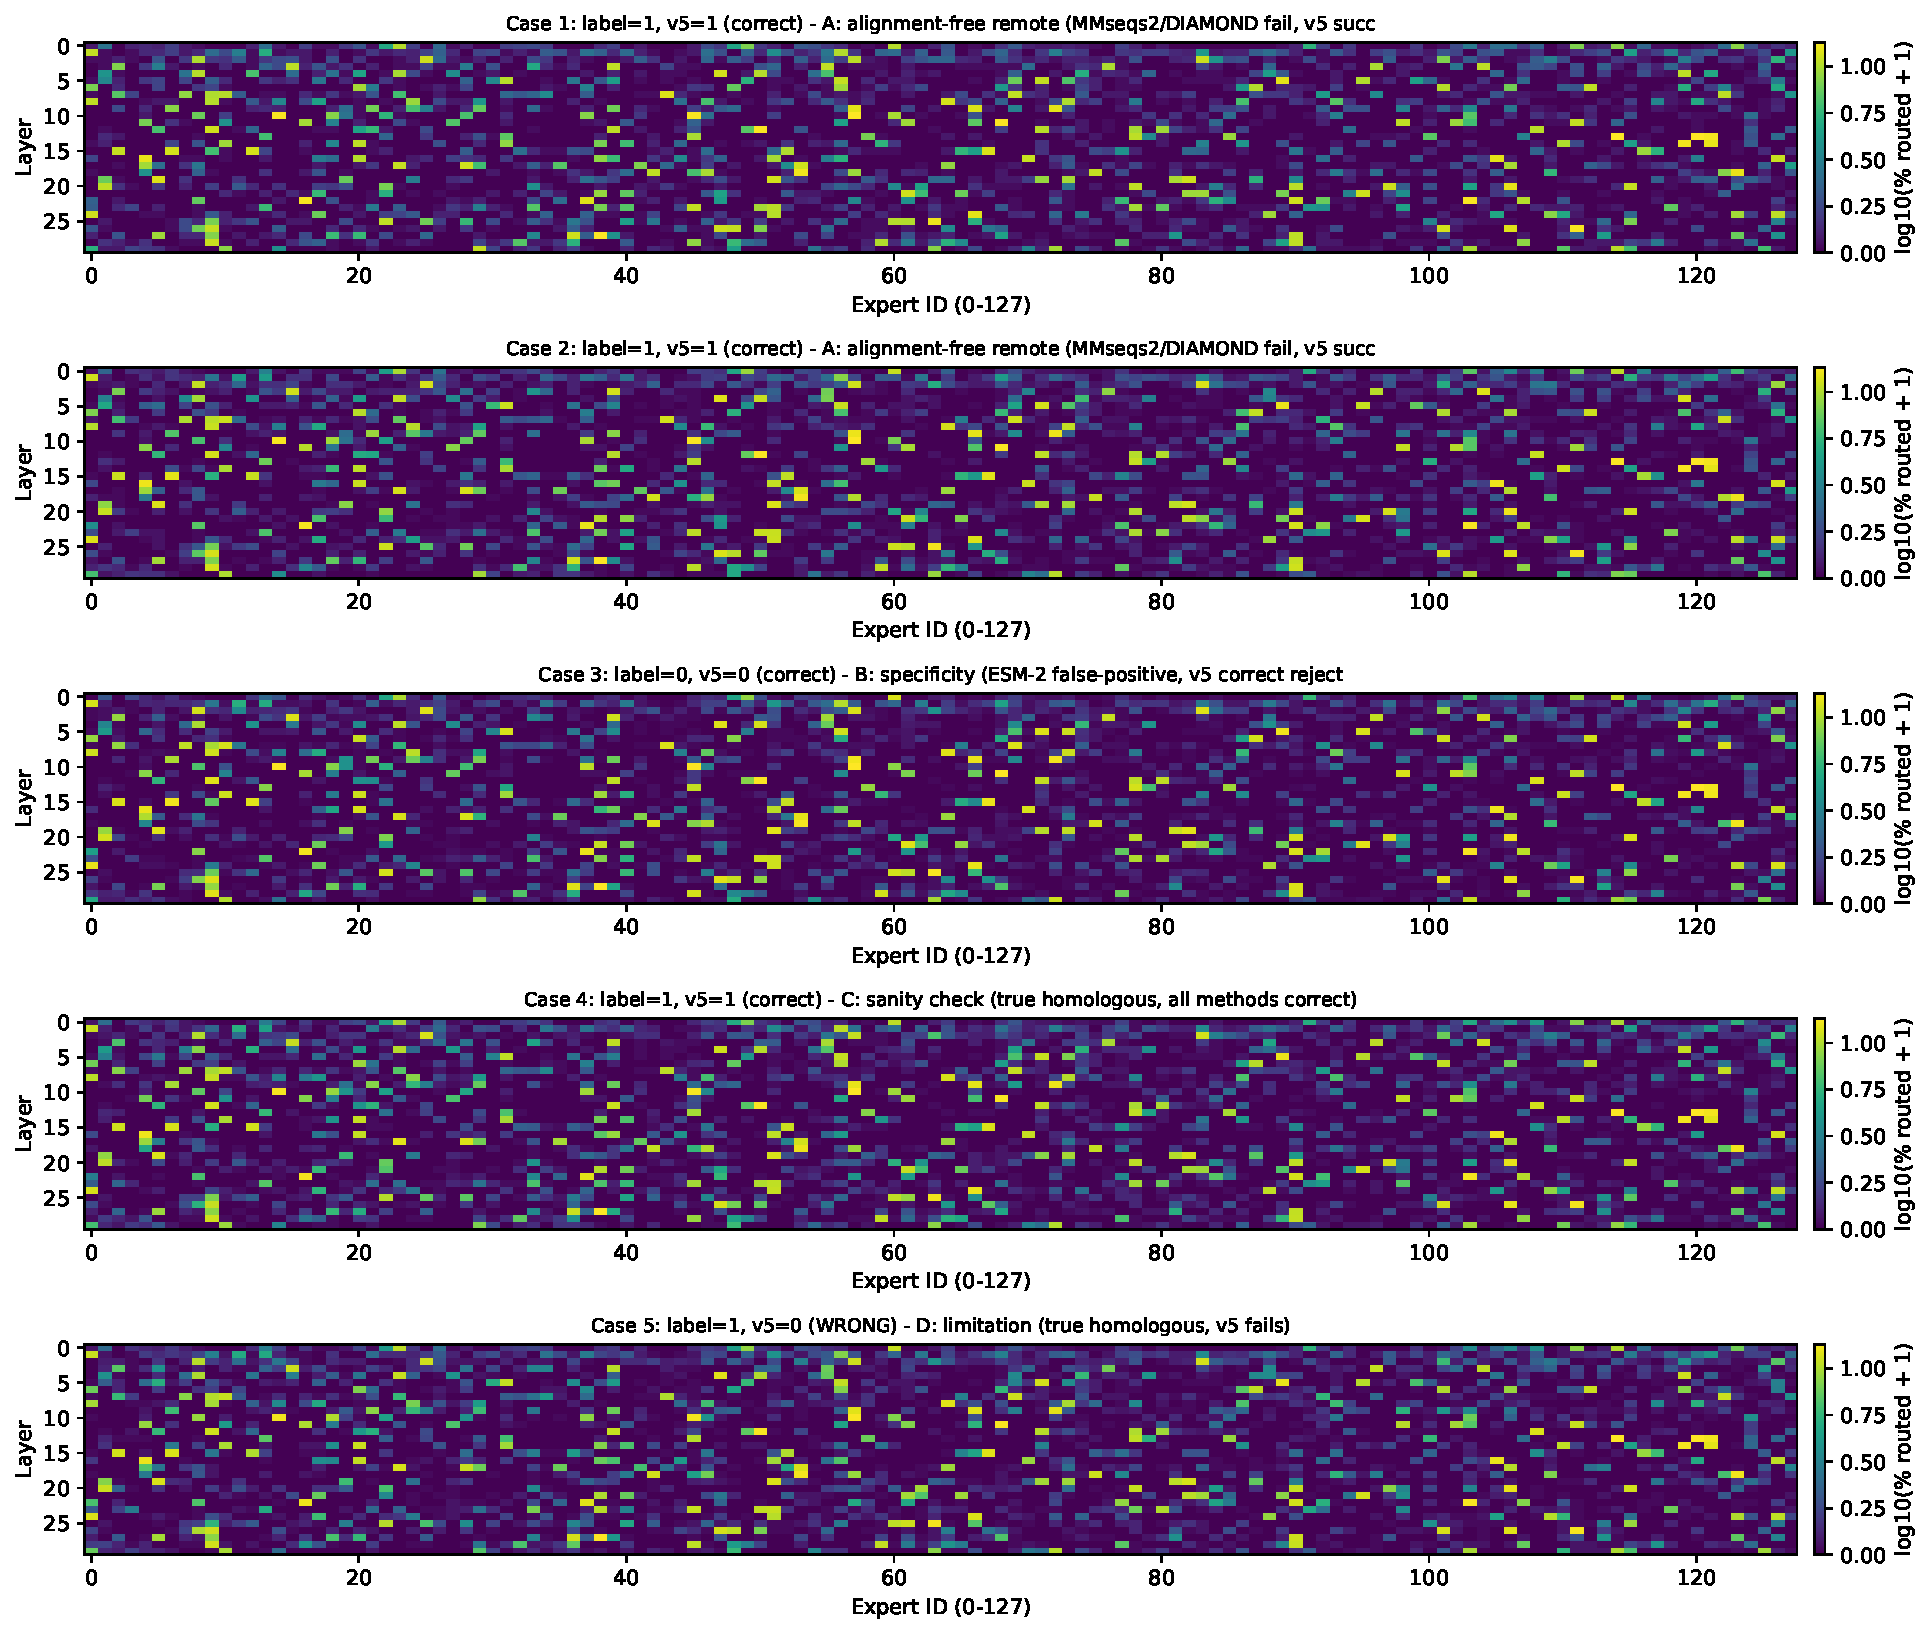
\includegraphics[width=0.95\textwidth]{figures/case_study_routing_mosaic.pdf}
\caption{Per-case routing-fraction matrix (30 layers $\times$ 128 experts), log-scaled. Visually similar across all five cases, with the strongest activation cluster near experts 0--20 and 100--115 in middle layers. Consistent with the protein-rich expert population identified in Table S11.}
\end{figure}

%% ============================================================
\section{Code and Model Availability}
%% ============================================================

All code, training scripts, and analysis notebooks are available at:
\begin{center}
\url{https://github.com/maris205/omnigene4}
\end{center}

\subsection{Key Scripts}

\begin{itemize}
\item \texttt{biopaws/cpt/1-prepare\_cpt\_data\_mp.py} -- CPT data preparation
\item \texttt{biopaws/cpt/2-run\_cpt.py} -- CPT training (8-GPU DDP)
\item \texttt{biopaws/sft\_data/17-train\_bio\_sft\_v3\_remote.py} -- SFT v3
\item \texttt{biopaws/cpt/40-train\_bio\_sft\_v4.py} -- SFT v4 (Alpaca + loss-mask)
\item \texttt{biopaws/cpt/41-train\_bio\_sft\_v5\_classifier.py} -- SFT v5 (dual-head)
\item \texttt{biopaws/cpt/43-eval\_v5\_full.py} -- v5 evaluation
\item \texttt{biopaws/cpt/44-merge\_v5\_to\_full.py} -- v5 LoRA $\to$ BF16 merge
\item \texttt{biopaws/cpt/50-esm2\_3b\_remote\_500pair.py} -- ESM-2 3B baseline
\item \texttt{biopaws/cpt/51-classical\_baselines\_500pair.py} -- MMseqs2/DIAMOND
\item \texttt{biopaws/cpt/52-collect\_per\_pair\_predictions.py} -- Per-pair collection
\item \texttt{biopaws/cpt/53-pick\_case\_studies.py} -- Case-study selection
\item \texttt{biopaws/cpt/54-extract\_routing\_heatmap.py} -- Router hook extraction
\item \texttt{biopaws/cpt/55-plot\_case\_studies.py} -- Figure generation
\end{itemize}

\subsection{Model Weights (Hugging Face)}

\begin{itemize}
\item \url{https://huggingface.co/dnagpt/OmniGene-4-CPT-v2-merged} -- CPT-only, BF16 ($\sim$50\,GB)
\item \url{https://huggingface.co/dnagpt/OmniGene-4-SFT-v3-merged} -- v3, BF16 ($\sim$50\,GB)
\item \url{https://huggingface.co/dnagpt/OmniGene-4-SFT-v3-GGUF} -- v3, Q4\_K\_M ($\sim$16\,GB)
\item \url{https://huggingface.co/dnagpt/OmniGene-4-SFT-v4} -- v4 LoRA ($\sim$1.9\,GB)
\item \url{https://huggingface.co/dnagpt/OmniGene-4-SFT-v5} -- v5 LoRA + heads ($\sim$1.9\,GB)
\item \url{https://huggingface.co/dnagpt/OmniGene-4-SFT-v5-merged} -- v5, BF16 + heads ($\sim$52\,GB)
\end{itemize}

\end{document}
